As said before in section \ref{sec:context_intro}, there's a clear lookout for automation
and easing management of the flows within logistics and the organisation came with
a solution to this problem, but as it's just an MVP, it's still missing some points
in terms of security, flexibility and rigidness.

To start off, an \emph{MVP} is a minimum viable product, which is a product that
is designed to be used in a limited number of situations and it's first aim
is providing an actual product to the customer and then use it to know learn
the behavior of the users and gain some understanding their interest \cite{MVP_def}.

\begin{figure}[h]
    \centering
    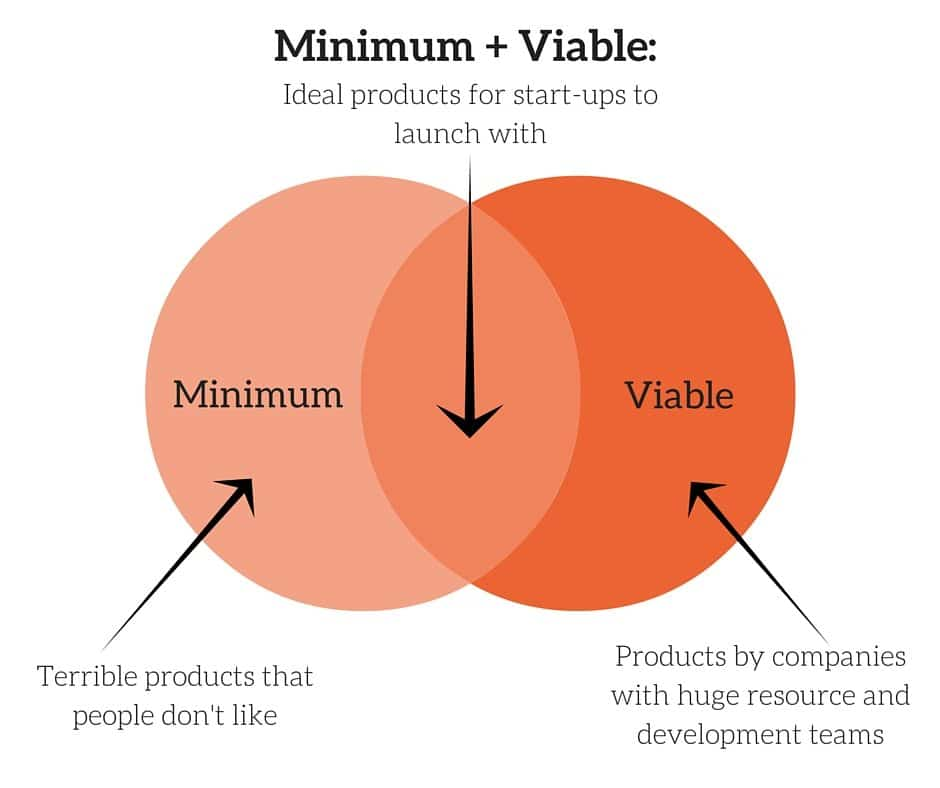
\includegraphics[width=0.6\textwidth]{images/Minimum-Viable.jpg}
    \caption{\footnotesize{Concept of a Minimum Viable Product - \cite{MVP_def}}}
    \label{fig:mvp}
\end{figure}

So going from this definition, it can be clear that a full fledged rigid
solution is never the aim of an MVP, but rather it's just a starting point
for a progressive and flexible solution and for the organization it came in
perfect as this application came in as a subject of a competition and
also the team is small so they didn't have the resources to finance
the creation of a big project. But going for the premise of building as you go,
but this came with it's own drawbacks, leading to a product stuck in the development
hell for too long as there are no clear guidelines for quality and security, so it's
not good once it takes too long and start becoming a costy solution to the creator
with no way to compete in the market.

So here comes the need to implement industrial standards and guidelines, which
is the aim for now, these standards are as follow:
\begin{itemize}
    \item \emph{Security}: Implement a security layer to protect the data
        and servers from unwanted visitors and attacks.
    \item \emph{Flexibility}: Creating a flexible solution, that's easy
        to use and extend by the client for their desired functions rather
        than having to develop and adapt the software each time.
    \item \emph{Maintainable}: Make the solution as easy to maintain,
        update and to pickup bugs.
    \item \emph{Automated deployment}: Make the solution deployable in an
        automated way, encouraging testability of the solution before it's
        deployed to any environment.
    \item \emph{Rigid solution}: Creating a solution as rigid as possible,
        so that it can tend to heavy load, have close to no down time and
        be more stable during peak times.
\end{itemize}

By implementing these standards, the solution can easily turn from an MVP to
a robust SaaS, which can be used in production and can be competitive in
the market.


